%!TEX root = main.tex

\chapter{Propositional Formulas and Models}

In this chapter, we start the discussion of propositional logic. We will define, how propositional formulas look, what is a model in propositional logic and we will also discuss some special forms of formula.

Propositional logic is the more basic type of logic (and predicate logic is an extension of propositional logic in a sense).  Propositional formulas (propositions) are created from so called \emph{propositional variables} that represent an atomic fact which can either be true or false. These propositional variables can only be connected by common logic connectives ($\to$, $\lequiv$, $\land$, $\lor$, $\neg$). Logical formulas can additionally use parentheses to indicate priorities of connectives. While the propositional formulas are simple compared to formulas in other types of logic, they are still useful. One of the most important problems in propositional logic and in computer science in general is the satisfiability of propositional formulas (SAT). Many other NP-complete problems are often solved by transformation to the SAT problem and using one of the existing SAT solvers.

The set of propositional variables is often called $\Prop$ and the variables themselves are usually named $p, q, r, s$ or $p_0, p_1, \dots, q_0, q_1$, or similarly. Now, we can formally define the propositional formula (over $\Prop$).

\begin{definition}
Let $\Prop$ is the set of propositional variables, than
\begin{enumerate}
  \item Every propositional variable from $\Prop$ is a propositional formula.
  \item If $\varphi$ and $\psi$ are propositional formulas, than $(\varphi \to \psi), (\varphi \land \psi), (\varphi \lor \psi), (\varphi \lequiv \psi)$, and $(\neg \varphi)$ are propositional formulas.
  \item Every propositional formula is created by finite application of the two rules above.
\end{enumerate}
\end{definition}

The last part of the definition ensures that every formula is finite, this also means that each formula can contain only a finite number of distinct variables. The set of propositional variables used in a formula $\varphi$ will be denoted as $\Var(\varphi)$. On the other hand, the set of all propositional formulas using only variables from a set $\Prop$ will be denoted as $\VF_\Prop$.

Formulas are thus strings of created from propositional variables, logical connectives, and parentheses, that fulfill the conditions in the definition above. A substring of such a string that also fulfills the conditions is called a \emph{sub-formula}. 

The formal definition of formula dictates the use of parentheses around every sub-formula, which can be rather cumbersome, therefore, we define priorities of the logical connectives and can thus omit some of the parentheses. The standard priorities are such, that the negation ($\neg$) has the highest priority (therefore parentheses around $(\neg \varphi)$ can always be omitted), conjunction and disjunction ($\lor, \land$) have ``middle'' priority, and implication and equivalence ($\to, \lequiv$) have the lowest priority. Therefore, we can write $\varphi \land \psi \to \neg \varphi \lor \xi$ instead of $((\varphi \land \psi) \to ((\neg \varphi) \lor \xi))$. 

Each formula can be also represented by a so called \emph{formation tree}, which is a finite ordered tree, whose nodes are labeled with propositions -- the leaves are labeled with propositional variables, if a node has label $(\neg \varphi)$, it has a single son labeled with $\varphi$, and if a node has label $(\varphi \to \psi), (\varphi \land \psi), (\varphi \lor \psi),$ or $(\varphi \lequiv \psi)$, it has two sons, the left one has label $\varphi$, and the right one has label $\psi$. For example, a formula $p \land q \to \neg (p \lor s)$ is represented by the formation tree on the left.
\begin{marginfigure}[-4\baselineskip]
\centering
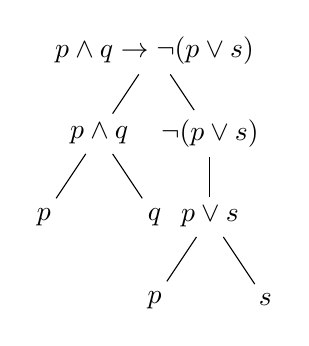
\begin{tikzpicture}[sibling distance=4em, level distance=3em]
  \node {$p \land q \to \neg (p \lor s)$}
    child { node {$p \land q$} 
      child {node {$p$}}
      child {node {$q$}} }
    child { node {$\neg (p \lor s)$}
    	child {node {$p \lor s$}
    		child {node {$p$}}
      	child {node {$s$}}}
     };
\end{tikzpicture}
\caption{The labeled ordered tree representing the formula $p \land q \to \neg (p \lor s)$.}
\end{marginfigure}

It is simple to show (by the induction on the number of nested parentheses) that each formula is associated with a unique formation tree. 

Once we have the formal definition of the formula (the syntax of propositional logic), we can define its semantics (what the formula means). The propositional variables represent atomic statements, that can have on of two truth values -- either 0 (false) or 1 (true). The truth value of the whole proposition in then given by the truth values of the variables and by the semantics of the logical connectives, which is given in Table~\ref{tab:prop_semantics} bellow.

\begin{table}[h]
\centering
\caption{The semantics of logical connectives}
\label{tab:prop_semantics}
\begin{tabular}{cc|ccccc}
\toprule
$p$ & $q$ & $\neg p$ & $p \lor q$ & $p \land q$ & $p \to q$ & $p \lequiv q$ \\
\midrule
0 & 0 & 1 & 0 & 0 & 1 & 1 \\
0 & 1 & 1 & 1 & 0 & 1 & 0 \\
1 & 0 & 0 & 1 & 0 & 0 & 0 \\
1 & 1 & 0 & 1 & 1 & 1 & 1 \\
\bottomrule
\end{tabular}
\end{table}

We can also consider the table above a definition of Boolean functions $\lor_1, \land_1, \to_1, \lequiv_1,$ and $-_1$, that implement the logical connectives. We will use these functions in cases where it is needed (e.g. while talking about truth values of propositions). More generally, any propositional formula with $n$ variables defines a Boolean function $f: \{0,1\}^n \to \{0,1\}$ (later, we will also see that any Boolean function can be expressed using a propositional formula).

We can now define the truth assignment and the truth value of formula more formally.

\begin{definition}
A \emph{truth assignment} is a function $v: \Prop \to \{0,1\}$, that is $v \in \fset{\Prop}{2}$.

A \emph{truth value} $\bar{v}(\varphi)$ of a propositional formula $\varphi$ for a truth assignment $v$ is defined inductively as:
	\begin{itemize}
		\begin{minipage}{0.5\textwidth}
		\item $\bar{v}(p) = v(p)$ if $p \in \Prop$
		\item $\bar{v}(\neg \varphi) = -_1(\bar{v}(\varphi))$ 
		\item $\bar{v}(\varphi \lor \psi) = \lor_1(\bar{v}(\varphi),\bar{v}(\psi))$ 
		\end{minipage}
		\begin{minipage}{0.5\textwidth}
		\item $\bar{v}(\varphi \land \psi) = \land_1(\bar{v}(\varphi),\bar{v}(\psi))$ 
		\item $\bar{v}(\varphi \to \psi) = \to_1(\bar{v}(\varphi),\bar{v}(\psi))$ 
		\item $\bar{v}(\varphi \lequiv \psi) = \lequiv_1(\bar{v}(\varphi),\bar{v}(\psi))$ 
		\end{minipage}
	\end{itemize}
\end{definition}

We can easily show (by the induction on the structure of the formula) that the truth value of a formula $\varphi$ depends only on the truth assignment of variables from $\Var(\varphi)$.

A proposition $\varphi$ over $\Prop$ is \emph{true in (satisfied by) an assignment} $v\in \fset{\Prop}{2}$, if $\bar{v}(\varphi) = 1$. In such a case, $v$ is called a \emph{satisfying assignment} for $\varphi$, we denote this fact $v \vDash \varphi$. If the formula is true for all assignments $v \in \fset{\Prop}{2}$, we say that it is \emph{valid (a tautology)} and denote the fact as $\vDash \varphi$. On the other hand, if there is no assignment for which the formula is true, it is called \emph{unsatisfiable (a contradiction)}. A formula $\varphi$ is \emph{independent (a contingency)} if it is neither a tautology nor a contradiction, i.e. there are two assignments $v_1, v_2 \in \fset{\Prop}{2}$, such that $\bar{v}_1(\varphi) = 1$ and $\bar{v}_2(\varphi) = 0$. Finally, a formula is \emph{satisfiable} if there is a truth assignment in it is true.

A truth assignment of $\Prop$ is also called a model of the language $\Prop$. The set of all models of $\Prop$ is denoted as $M(\Prop)$, and, obviously $M(\Prop) = \fset{\Prop}{2}$. A proposition $\varphi$ over $\Prop$ is valid in a model $v \in M(\Prop)$, if $\bar{v}(\varphi) = 1$. Then we also say that $v$ is a model of $\varphi$, denoted as $v \vDash \varphi$. $M^\Prop(\varphi) = \{v \in M(\Prop) | v \vDash \varphi\}$ is the \emph{class of all models} of $\varphi$. A formula is valid, if it is true in every model of the language, it is unsatisfiable if it does not have a model, and satisfiable if it has a model. It is independent if it is true in a model of the language and false in another one. Formulas $\varphi$ and $\psi$ are logically equivalent ($\varphi \sim \psi$, if $M^\Prop(\varphi) = M^\Prop(\psi)$.

The last two paragraphs say basically the same, the difference is that in the latter one, we use the notion of model, which is central to logic. The notion of models, and sets of models will be important later, and ``model'' is one of the key term in logic.

In the definition of propositions, we used 5 different logical connectives. However, if we take a look at the table with their semantics, we may notice, that, for example, $p \to q$ is equivalent $\neg p \lor q$. Therefore, even without using the implication ($\to$) we can still express everything we could with them. More formally, for every formula $\varphi \in \VF_\Prop$, there is an equivalent formula $\varphi'$ that does not use the implication. Moreover, we can notice, that $p \lequiv q$ is equivalent to $(p \to q) \land (q \to p)$, therefore we even do not need the equivalence, and every formula can be written using only negation, conjunction, and disjunction ($\neg, \land, \lor$). This feature of the set can be defined more formally.

\begin{definition}
A set of connectives is \emph{adequate} if they can express any Boolean function by some proposition from them.
\end{definition}

We have already discussed that the set ($\neg, \land, \lor$) is adequate. We can also show, that the set $\{\to, \neg\}$ is adequate, the easiest way to do that is to realize, that $(p \land q) \sim \neg (p \to \neg q)$ and $(p \lor q) \sim (\neg p \to q)$. 

Generally, we can also define custom connectives, for example, the so called Shaffer stroke (NAND) is defined as $p \uparrow q \sim \neg (p \land q)$, or the Pierce arrow (NOR) is defined as $p \downarrow q \sim \neg (p \lor q)$. Interestingly, both $\{\uparrow\}$ and $\{\downarrow\}$ are adequate sets. This is an important fact for the construction of logical circuits as we can use a logical gate of only one kind (either NAND or NOR) to express any Boolean function.

There are also special forms of formulas, which are often used. Among the most common ones are so called conjunctive and disjunctive normal forms. In order to define these two forms, we first need to define a literal. A \emph{literal} is a propositional variable or its negation, for example, if $\Prop = \{p, q\}$ then all the literals we can construct over $\Prop$ are $\{p, \neg p, q, \neg q\}$. A formula is in conjunctive normal form (CNF) if it is a conjunction of disjunctions of literals. Disjunctions of literals are also called \emph{clauses}, therefore we can also say, that a CNF formula is a conjunction of clauses. On the other hand, a formula is in disjunctive normal form (DNF) if it is a disjunction of conjunctions of literals. So, for example, $(p \lor \neg q \lor r) \land (p \lor q) \land (\neg p \lor q \lor r)$ is a formula in CNF and$(\neg p \land q \land \neg r) \lor (\neg p \land \neg q) \lor (p \land \neg q \land \neg r)$ is a formula in DNF (and, moreover a negation of the previous one in CNF). 

Now, we would like to show, that for every formula, there is an equivalent formula in CNF and another equivalent formula in DNF. To this end, we will need to following set of rules, which can be proved manually by checking the truth table of the propositional connectives: 

\begin{enumerate}
  \item $(\varphi \to \psi) \sim (\neg \varphi \lor \psi), (\varphi \lequiv \psi) \sim ((\neg \varphi \lor \psi) \land (\neg \psi \lor \varphi))$
  \item $\neg \neg \varphi \sim \varphi, \neg (\varphi \land \psi) \sim (\neg \varphi \lor \neg \psi), \neg (\varphi \lor \psi) \sim (\neg \varphi \land \neg \psi)$
  \item $(\varphi \lor (\psi \land \chi)) \sim ((\psi \land \chi)  \lor \varphi) \sim ((\varphi \lor \psi) \land (\varphi \lor \chi))$
  \item $(\varphi \land (\psi \lor \chi)) \sim ((\psi \lor \chi)  \land \varphi) \sim ((\varphi \land \psi) \lor (\varphi \land \chi))$
\end{enumerate}

We can also easily show (again by induction on the structure of the formula) that if we have a formula $\varphi'$ which is obtained from $\varphi$ by replacing some occurrences of its sub-formula $\psi$ with an equivalent sub-formula $\psi'$, then $\varphi \sim \varphi'$.

And finally, we can show the following theorem. 

\begin{theorem}
For every formula $\varphi$ over $\Prop$, there are formulas $\varphi_C$ and $\varphi_D$, such that $\varphi_C$ is in CNF, $\varphi_D$ is in DNF and $\varphi \sim \varphi_C$ and $\varphi \sim \varphi_D$.
\end{theorem}
\begin{proof}
The propositions $\varphi_C$ and $\varphi_D$ can be obtained from $\varphi$ by applying the rules 1 to 4 mentioned above. 
\end{proof}

The discussion above shows one of the ways to obtain equivalent formulas in CNF and DNF to a given formula. We can in fact apply the rules in the order, in which they are presented. First, we remove all the implications and equivalences by using the rules no. 1. Then, we move all negations to the literals (i.e. there are no negations outside of parentheses), using the rule no. 2 and, finally, we repeatedly apply rules no. 3 and 4 to obtain the CNF and DNF. 

This syntactic approach is not the only one to obtain CNF/DNF from a given formula. We can also construct the truth table of the formula and then read the CNF/DNF almost directly from the table. We will show a more general approach here, we will construct a CNF and DNF formulas $\varphi_C$ and $\varphi_D$ such that $M^\Prop(\varphi_C) = M^\Prop(\varphi_D) = K \subseteq M(\Prop)$, for a given finite set of truth assignments $K$. 

Before we show the construction, we will define the notion of $p^t$ for a variable $p$ and a truth value $t$ as $$ p^t \twopartdef{p}{t = 1}{\neg p}{t = 0}\,.$$ 

Now, we can easily see that for a single assignment $v \in K$, the set of models of the formula $\Land_{p \in \Prop} p^{v(p)}$ contains only $v$. For a set of assignments $K$, we can just make a disjunction over all assignments in $K$ (remember $K$ is a finite set). Therefore, $$M(\Lor_{v \in K}\Land_{p \in \Prop}p^{v(p)}) = K\,.$$ Thus we constructed a formula in DNF whose models are exactly the set $K$. 

Constructing a formula $\varphi$ in CNF such that $M(\varphi) = K$ for some given finite $K$ is slightly more complex. However, we can use the fact that the negation of a formula in DNF is a formula in DNF. Negating a formula in CNF means changing all the conjunctions to disjunctions and vice versa and changing all literals to the complementary ones (i.e. changing $p$ to $\neg p$ and vice versa). So, we start by creating a formula $\neg \varphi$ in DNF for the set $\fset{\Prop}{2} \setminus K$ according to the approach above. Then, we negate the formula, thus obtaining $\varphi$ in CNF such that $M(\varphi)=K$. Following these two steps we obtain the formula $$\varphi = \Land_{v \in \fset{\Prop}{2} \setminus K}\Lor p^{-_1v(p)}$$ such that $M(\varphi) = K$.

If we want to use this approach to create a formula in CNF or DNF equivalent to a formula $\varphi$, we simply choose $K=M(\varphi)$. This description also shows that any Boolean function $f$ (i.e. function $f: \{0,1\}^n \to \{0,1\}$) can be expressed as a proposition. We can choose $K = \{v | f(v) = 1\}$. 

Both the techniques described above lead to an equivalent formula in CNF/DNF. Choosing the better one for the task depends on a few features of the ``input'' formula. Typically, the table-based method is preferred for formulas with only a few variables (as the size of the table grows exponentially with the number of variables). 
